\documentclass[man,noapacite,12pt]{apa2}
\usepackage{amsmath}
\usepackage{booktabs}
\usepackage{apacite2}
\usepackage{fullpage,rotating}
\usepackage{pslatex}
\usepackage{amssymb}
\usepackage{accents}
\usepackage{xcolor}
% \usepackage{caption}
% \usepackage{subcaption}
\usepackage{graphicx}
% \captionsetup{compatibility=false}

% \usepackage{synctex}

\newcommand{\vect}[1]{\accentset{\rightharpoonup}{#1}}

\newcommand{\nnote}[1]{\textcolor{blue}{[#1]}}


\title{Learning word meaning by inferring speakers' intentions: \\ An incremental approach to socially-guided statistical learning}

\author{Michael C. Frank, Molly L. Lewis, Mika Braginsky, \& Noah D. Goodman}
\affiliation{Department of Psychology, Stanford University}

\shorttitle{Learning words by inferring reference}
\rightheader{Learning words by inferring reference}


\acknowledgements{Many thanks to ...

~

\noindent Please address correspondence to Michael C. Frank, Department of Psychology, Stanford University, 450 Serra Mall (Jordan Hall), Stanford, CA, 94305, tel: (650) 724-4003, email: \texttt{mcfrank@stanford.edu}.}


\abstract{How do children learn the meanings of words? Some accounts suggest that word learning happens in a single moment, while others privilege the gradual accumulation of information across time. Previous modeling work has attempted to unify these viewpoints in a single framework that allows for both in-the-moment interpretation and gradual statistical accumulation, but at the cost of substantial computational complexity. We describe a new, incremental model of this interaction, in which statistical associations are the product of in-the-moment interpretations. This process-level model successfully captures a number of experimental findings and suggests a number of extensions.}

\begin{document}
\maketitle                            


\section{Introduction}

Word learning is a foundational part of language acquisition. Starting slowly in late infancy and speeding up after their first birthday, children accumulate a vocabulary of words that they can reliably recognize and produce \cite{bergelson2012,bloom2002}. The exact timing of this process is highly variable across children, but generally by the end of the second year, children can produce several hundred words and are well on their way to combining these to express complex and novel propositions \cite{brown1973,fenson1994}. How are these early words learned? 

In this paper, we elaborate an answer to this question that combines children's statistical learning abilities \cite{saffran1996b,aslin2012} with their emerging competence in social interaction \cite{carpenter1998}. Our proposal is that vocabulary is accumulated via a process in which children attempt to interpret the language they hear. In this proces of interpretation, children make guesses---some more secure than others---about the meanings of words, which they then retain to guide future interpretation. Building on a previous model of joint interpretation and language learning \cite{frank2009}, we implement this proposal in the language of probabilistic modeling. Our model instantiates the idea that there are two timescales involved in word learning \cite<cf.>{mcmurray2012}: in-the-moment interpretation and cross-situational mapping. 

Our model constitutes an incremental approach to integrating across timescales: For each utterance, it proposes a possible referential interpretation, then updates a graded lexicon accordingly. Although the model is incremental, it nevertheless instantiates normative Bayesian inferences; in this respect it is a ``rational process model'' that makes normative probabilistic inferences under cognitive resource constraints \cite{griffiths2012,sanborn2010}. We compare this incremental, process-level inference algorithm with a batch inference algorithm that considers all the available data and find that they are surprisingly similar to one another. One somewhat radical consequence of this approach is that there is no separate process of ``word learning''; instead word learning is what falls out of learners remembering their best guesses about what a particular piece of language meant in the contexts of its use.

In what follows, we motivate our proposal with respect to the previous literature on children's word learning. We then review prior computational models of word learning with the goal of grounding and highlighting our conceptual contributions. We next present our model and show that it can be both applied to annotated corpora of child language and can be used to simulate individual experiments. We end by considering open questions for the field of early word learning.

\subsection{Mechanisms of early word learning}

One clue to the mechanisms of early vocabulary learning comes from the makeup of children's early vocabulary. Although children produce words of all different types, certain kinds of words are nevertheless overrepresented in early vocabulary. Names for things make up a substantially larger proportion of children's early vocabulary than they do later \cite{tardif2008,caselli1995}, alongside names for people and and words used in simple social routines (e.g., ``hi'' and ``bye''). Many observers have suggested that these kinds of words---especially basic-level nouns---are learned early because of the ease with which the linguistic form can be mapped to a particular observable referent \cite{locke1700,bloom2002,clark2003}. From there, generalizing particular referents to a broader class of referents is relatively trivial, given that the relevant concepts are typically at the basic-level and typically represent whole objects rather than parts \cite{markman1991}.

A single learning instance can in principle provide strong evidence for a particular word meaning. For example, imagine that a parent points to a ball and says ``ball'' An observer with an understanding of pointing can infer that the speaker is referring to the ball, infer that the concurrently uttered word refers to it, and generalize to the broader concept of balls in general. In practice, however, very young children typically require at least a handful (and often far more) exposures to a word before they recognize it and retain it for future use, even when the context of naming is unambiguous \cite{woodward1994}.

In addition, many learning situations range from slightly to substantially more ambiguous. Imagine that the parent had uttered the phrase ``look at that nice, round ball!''---this phrase has a number of competing words that might be candidates for the object name (though perhaps worse candidates by virtue of sentential position, stress, or phonological structure). Or the parent might not have pointed but instead relied on the fact that the child was playing with the ball. Perhaps there might have been other toys present competing for the child's attention. In each of these cases, the child might be able to guess that the word ``ball'' referred to the ball, but with less certainty than in the simplest case (\citeNP{gillette1999} and \citeNP{yurovsky2013} give concrete instantiations of such differences in certainty in naturalistic play session videos). 

Many theorists have noted that learners in principle could accumulate information across many ambiguous naming instances \cite{pinker1984,gleitman1990,siskind1996,yu2007}. This strategy, dubbed \emph{cross-situational learning}, has now been demonstrated in a number of small-scale laboratory experiments with both adults and children \cite{yu2007,smith2008}. In addition, a number of computational demonstrations suggest that this kind of strategy could be effective for learning in social situations \cite{yu2007b,frank2009,johnson2012}, with realistic vocabulary sizes and levels of ambiguity \cite{blythe2010}, and even with more complex propositional meanings \cite{siskind1996}. In fact, a growing literature in natural language processing implements precisely this strategy for a variety of what are known as ``grounded language learning'' tasks \cite<e.g.>{zettlemoyer2005,wong2007,artzi2013,liang2011,kim2013}.

Nevertheless, the existence of such an uncertainty-reduction strategy does not necessarily imply that learners make use of it. Indeed, there has been substantial debate about the degree to which learners represent cross-situational statistics \cite{medina2011,yu2012,yurovsky2013,trueswell2013,smith2011b,yurovskyunderreview}. On some accounts, learners encode only a single hypothesis at a time; on others, learners maintain some representation of all of the data that they have access to. But regardless of the specific representation and algorithm that learners use for this process, all accounts of cross-situational learning posit \emph{consistency} across situations, which even single-hypothesis learners exploit by checking their hypotheses across situations \cite{trueswell2013,yu2012}. To understand the range of possible theories of cross-situational learning, we next turn to the modeling literature. 

\subsection{Prior modeling work}

Although a number of theorists had discussed cross-situational strategies for learning word meanings \cite{pinker1984,gleitman1990}, an important early instantiation of this idea came from a model by \citeA{siskind1996}. This model used a propositional representation of meaning in combination with a set of deductive rules to infer word-meaning mappings from artificial data. This ambitious model provided a powerful proof-of-concept, but was limited by the assumption that the propositional structure of meanings was observed by the learner. 

An alternate, more graded, view of word learning came from the connectionist tradition. \citeA{plunkett1992} described a graded word-image mapping model that reproduced a number of category generalization and vocabulary growth phenomena. This basic model type has been followed by a number of related models that capture phenomena like mutual exclusivity \cite{regier2005}, the phonological dynamics of the mono- and bilingual lexicon \cite{li2002,li2004,li2007}, and the emergence of categorization principles \cite{mayor2010}. Though these models provide a powerful example of the emergence of a range of phenomena from a simple architecture, none focused specifically on the challenge of disambiguating reference in ambiguous contexts. 

The problem of referential uncertainty played a more central role in a number of other models that emerged from the machine learning tradition. In a series of investigations, Yu and colleagues developed a model stemming from classic machine translation systems \cite{brown1993}. This model looked for correspondences between words and their referents that was consistent across situations; these mappings could be biased by a number of perceptual and social aspects of the learning scenario \cite{yu2005,yu2007}. Critically, this model could be applied to annotated corpora of child-directed speech, a major advance over previous work that had only been used to learn from artificial corpora. 

A complementary model used the Bayesian framework considered how generalization biases could emerge from statistical inferences under ambiguity across situations \cite{xu2007}. This model was able to predict adults' and children's patterns of taxonomic generalization by reference to general principles of probabilistic inference. Although it did not specifically apply to the problem of referential uncertainty across situations, it nevertheless aggregated information across exposures to make graded inferences about word meaning. 

Building on these two lines of work, we proposed a probabilistic treatment of referential uncertainty in \citeA{frank2009}. This model differed from earlier approaches in that it explicitly assumed that in any individual situation, speakers have an intention to refer to a particular object or objects and that the labels they utter correspond to these words. In contrast, previous models had computed associations directly between words and referents, without considering that some of these associations were not relevant because the speaker might not be trying to refer to some objects. This ``intentional'' assumption led to an increase in accuracy in learning from corpus data relative to previous work, and also allowed the model to capture a number of experimental findings. A number of related pieces of work have extended this model to incorporate word segmentation \cite{johnson2010}, social cues \cite{frank2008,johnson2012}, conceptual generalization \cite{lewis2013b}, lexical constraints \cite{lewis2013}, bilingual lexica \cite{zinserunderreview}, some basic aspects of grammatical structure \cite{johnson2010}, and even pragmatic inference \cite{smith2013}.

The basic framework described in \citeA{frank2009} nevertheless suffered from a number of weaknesses. First, it posited a discrete lexicon represented by a bipartite graph linking words and object concepts. While this representation was technically convenient, it seemed at odds with the conception of graded, uncertain mappings implied by the experimental literature.\footnote{Although there is debate about the uncertainty implied by adult cross-situational learning experiments \cite<e.g.>{smith2011b,trueswell2013}, many experiments with children imply increases in word recognition accuracy with greater experience \cite<e.g.>{fernald1998,bergelson2012}. Some sort of graded conception of the lexicon appears to be an important aspect of models that hope to capture such findings.} In addition, the model was posed at Marr's \citeyear{marr1982} ``computational theory'' level; as such, it considered all the available data in its computation. This ``batch'' inference was of course unrealistic in terms of the memory constraints on leaners; in addition, practically speaking it kept the model from considering phenomena that involved the gradual accumulation of data about a particular inference. Finally, because of technical limitations, the inference scheme in this model was not fully Bayesian: It did not recover the posterior probability distribution on lexicons given a particular exposure. Instead, it only searched for the single best lexicon. 

Two other recent models have made progress in using incremental inference to describe word learning. First, \citeA{fazly2010} proposed an incremental version of the \citeA{yu2007} translation model, which they applied to meaning representations derived from speech in CHILDES. This model reproduced a number of empirical findings in the incremental context. In addition, the meaning representations were graded distributions over the full inventory of lexical elements. Both of these desirable features pointed the way towards further applications, and this basic model has been extended to simulate cognitive constraints \cite{nematzadeh2012}, individual differences in acquisition \cite{nematzadeh2011}, and the effects of syntactic structure \cite{alishahi2010}. One weakness of this work, however, is that this model has no obvious route for the accommodation of social information. 

Second, \citeA{mcmurray2012} introduced a connectionist model that---like the \citeA{frank2009} model---explicitly operates at two timescales: the timescale of language interpretation in the moment and the timescale of cross-situational mapping. Because of the incremental nature of this model, however, it was able to simulate the dynamics of reference resolution in the moment. In addition, the exhaustive set of simulations using this model suggests that the combination of graded representation, incremental processing, and multi-timescale inference allows this model to captures most of the relevant data points. Similar to the \citeA{fazly2010} model, however, the one major lacuna in this set of simulations is social learning phenomena. 

\subsection{The current model}

Taken together, the models presented by \citeA{frank2009}, \citeA{fazly2010}, and \citeA{mcmurray2012} synthesize and unify a striking amount of work on the mechanisms and dynamics of early word learning. Each of these has some features that could be improved upon, however. In particular, the \citeA{frank2009} model is non-incremental, while the \citeA{fazly2010}, and \citeA{mcmurray2012} models fail to consider social information. Our goal in the current work is thus to provide an incremental interpretation of the \citeA{frank2009} model, which would serve to unify the social framework in that work with the findings of these other incremental models.

\section{Model}


In the sections that follow, we describe the formal specification of our model as well as two inference algorithms---a batch Gibbs sampler and an incremental particle filter---that are focused around referential interpretation. As will become clear, these two inference algorithms are deeply related to one another. All code and data for the model and simulations reported below are available at \url{http://github.com/mcfrank/dmww}. 


%%%%%
%;;for reference, a church version of the dmww generative model... 
%(define words '(A B C D E F G H))
%
%(define lex (DPmem 1.0 (lambda (obj) (uniform-draw words))))
%;; (define lex (mem (lambda (obj) (make-dirichlet-multinomial langsize))))
%
%(define (sentence objs numwords) 
%  (define intent (uniform-draw objs))
%  (define ref (sample-integer (+ 1 numwords))) ;;ref = numwords+1 is if nothing is referential
%  (map (lambda (index)
%         (if (= index ref)
%             (lex intent)
%             (lex 'nonref)))
%       (range 0 (- numwords 1))))
%%%%%

\begin{figure}[tr]
\begin{center}
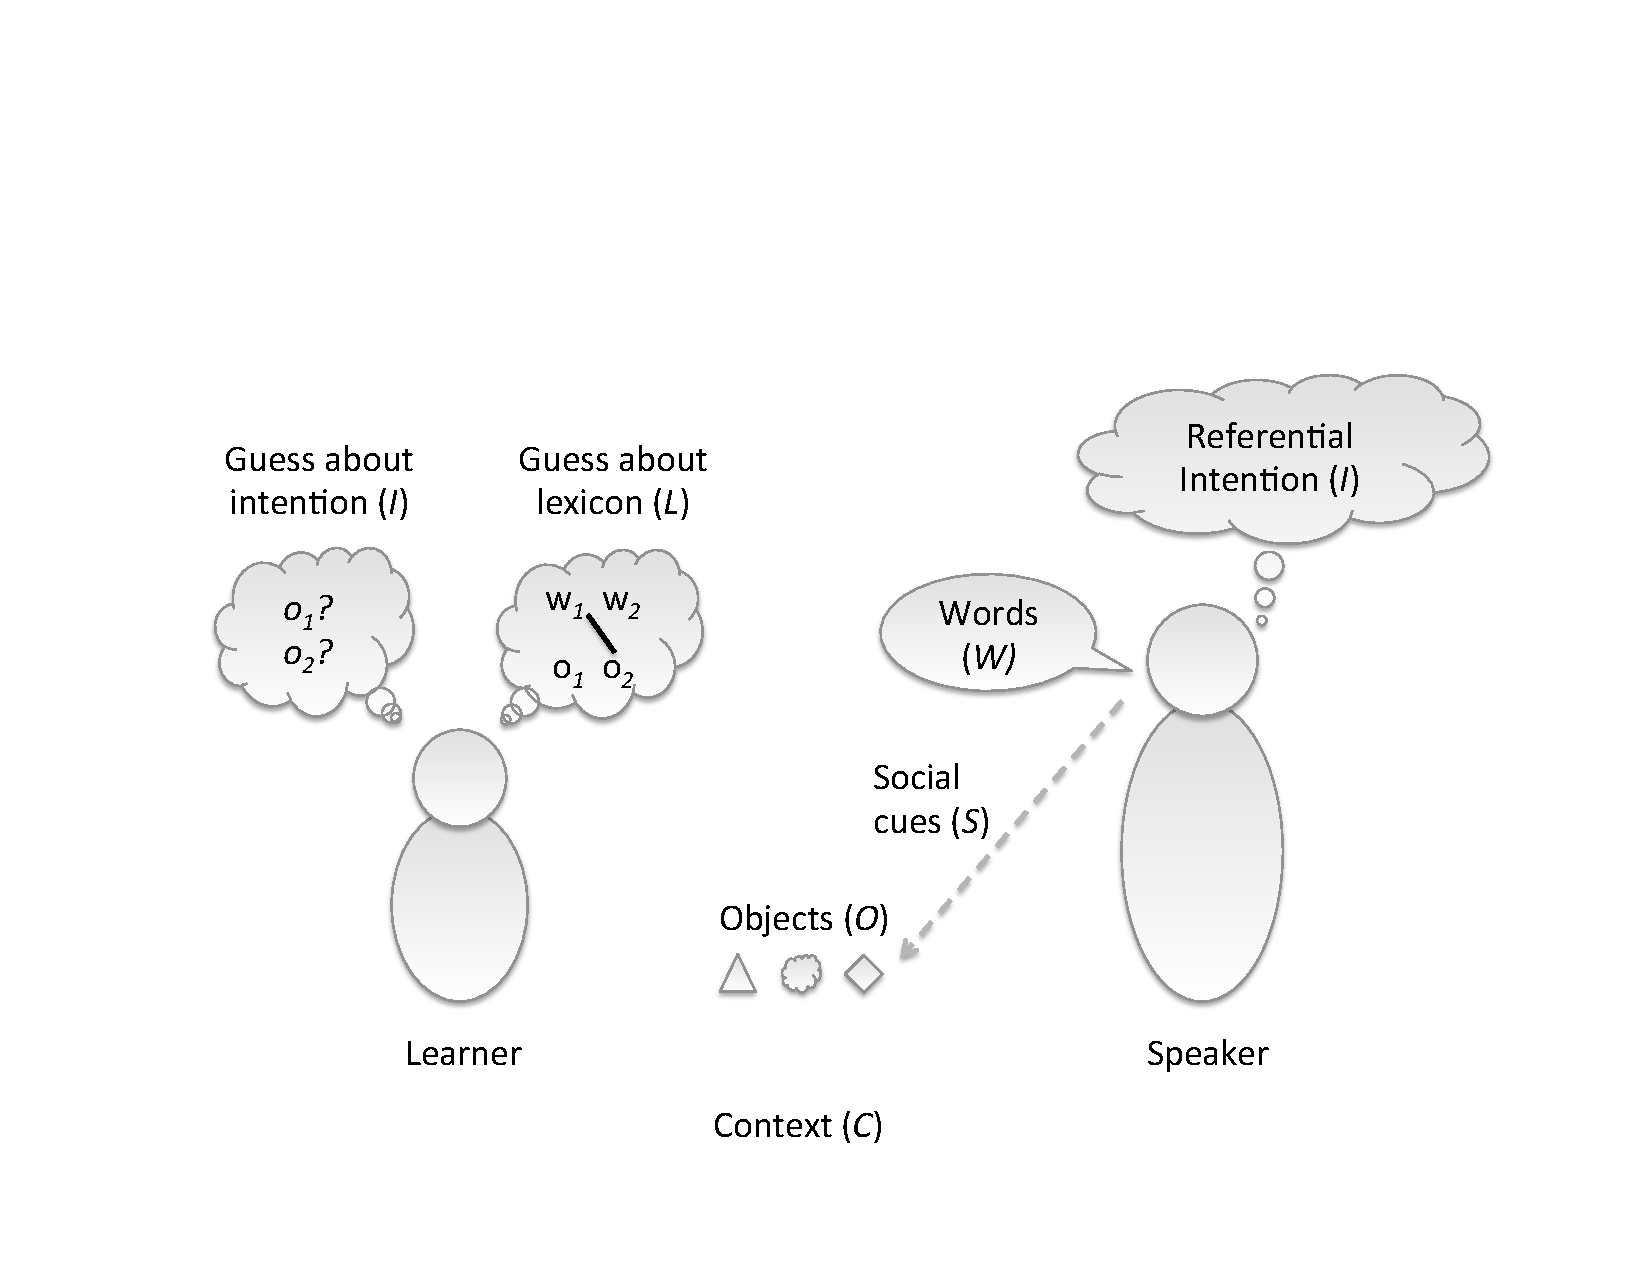
\includegraphics[width=4.5in]{figures/framework_mod.pdf}
\caption{\label{fig:setup} A schematic depiction of the learning situation, with the relevant variables marked for ease of interpretation. The learner faces a joint inference problem: inferring what the speaker is talking about and learning the consistent meanings of words. Reprinted from \protect\citeA{frank2014chap}.}
\end{center}
\end{figure}

The schematic word learning situation is shown in Figure \ref{fig:setup}. The learner is hypothesized to jointly infer the speaker's referential intention, $I$, and the lexicon of their language, $L$. These inferences are informed by the elements of the context, $C$: the words, $W$, that the speaker utters, the relevant referents (objects $O$) that are present in the situation, and potentially auxiliary social cues.

\subsection{The generative model}

A sketch of the generative model is shown in Figure \ref{fig:genmod}. We will write $\vec{W}$ for all utterances across contexts, $W^{i}$ for the utterance in the $i$th context, and $W^{i}_{j}$ for its $j$th word; similar for other variables.

\begin{figure}[tr]
\begin{center}
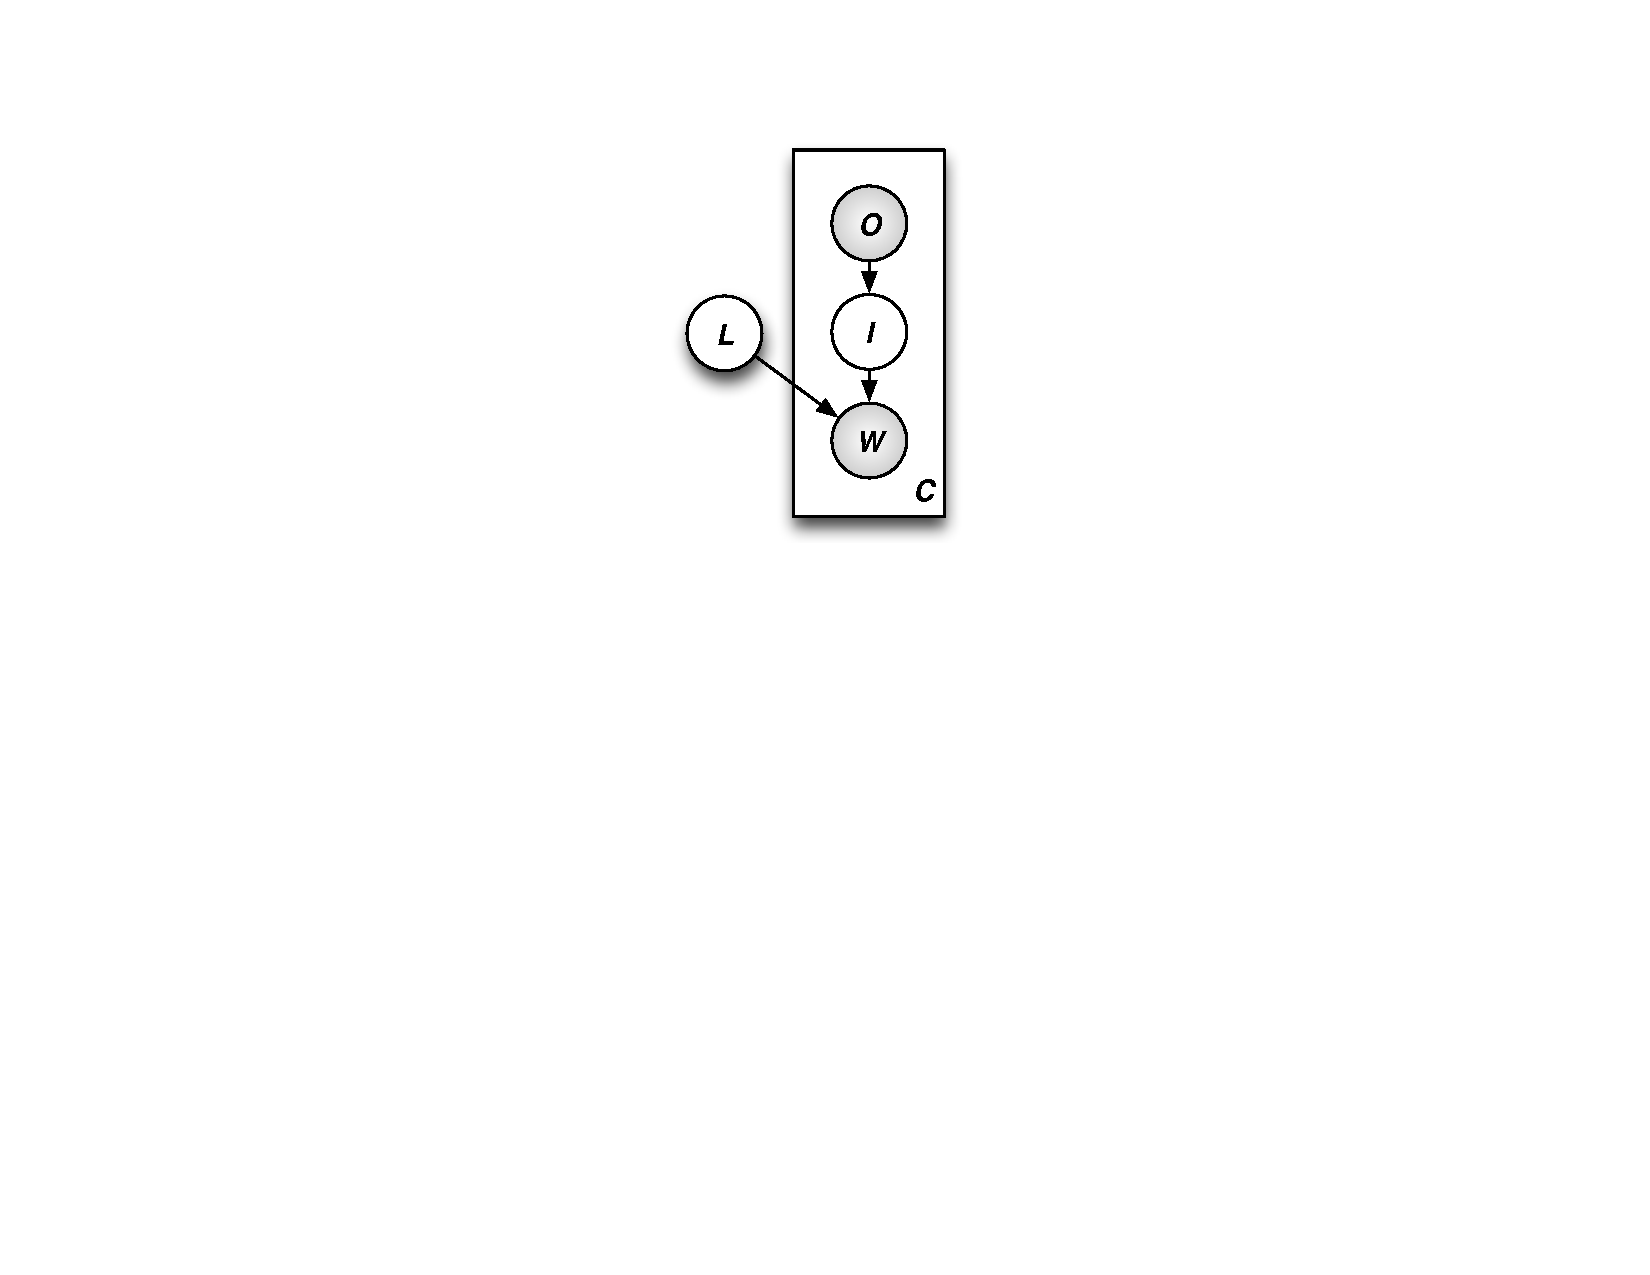
\includegraphics[width=1.5in]{figures/gen_mod.pdf}
\caption{\label{fig:genmod} The generative model assumed in our current work, similar to \protect\citeA{frank2009}. The plate over contexts indicates that objects, words, and referential intentions are present in each context, while the lexicon stays constant across contexts. \nnote{should update this fig with reference variables... also not currently mentioned in main text.}}
\end{center}
\end{figure}

Our primary departure from \citeA{frank2009} is to assume that the lexicon places a distribution over all words for each object, rather than being a discrete association from objects to words. That is, we smooth the previous model by allowing some probability that an unusual word is used to refer to an object. Formally we assume each the lexical entry for each object (type) is a distribution over words drawn from a symmetric Dirichlet distribution:
\begin{equation}
\label{eqn:lexprior}
L_{ob} \sim \text{Dirichlet}(\alpha)
\end{equation}
Where $ob$ can be any object in the world and can also be the special ``object'' $NR$, which accounts for all non-referential words.\footnote{We continue to discuss the model as linking words with \emph{objects}, rather than with \emph{concepts}. \citeA{lewis2013b} describes the generalization of a related model to learning category generalizations. Since the data we consider here are annotated for objects rather than concepts, the difference is purely rhetorical; but concepts are clearly the right units of generalization for future work.}
The words themselves will be drawn below from multinomial distributions with parameters determined by $L_{ob}$.

Following \citeA{frank2009} we assume that speakers have simple intentions to refer to objects in the context. For current purposes we simplify by assuming speakers intend to refer to only one object, and that they will refer to each possible object with equal probability. Thus $I^{i} \in O^{i}$ and
$P(I^{i}| O^{i}) = \frac{1}{|O^{i}|}$.
\nnote{This is where we put social cues.. either intention directly depends on social cues, $P(I^{i}| O^{i},S^{i})$, or social cues depend on intention, which still leads to a distribution on intentions that depends on social cues.}

We next assume that speakers realize their intention by deciding which word in the utterance should be the referring word, generating this word appropriately using the lexicon, and then generating ``non-referring'' words for the remainder of the utterance. \footnote{This is a departure from \citeA{frank2009} where it was assumed that each word might refer to an object independent of whether anther word also referred to that object. That is, here we assume that the pressure to refer can be ``satisfied'' by one word, leaving the other words to play other (non-referential) roles.}
That is, for an utterance of $N_{i}$ words there is a variable $r^{i} \in \{1,\dots,N_{i}, \emptyset \}$ that determines which word realizes the referential intention. The probability that $r^{i}=\emptyset$ (i.e.~no word realizes the referential intention) is a fixed constant, and $r^{i}$ has equal probability for the other words.
Words are then drawn from either the distribution specified by the lexicon for the intention object or the $NR$ non-referential item:
\begin{equation}
W^{i}_{j} \sim 
\begin{cases}
\text{Multinomial}(L_{I^{i}}) & \text{if } r^{i}=j \\
\text{Multinomial}(L_{NR}) & \text{otherwise}
\end{cases}
\end{equation}
Note that for any $j$, $\emptyset \neq j$ and as a result \emph{no} word in the utterance is referring when $r^{i}=\emptyset$.
% \nnote{do we need to give $P(W^{i}_{j}|...)$ or is the stats notation enough?}

The words in the utterance are independent given $r^{i}$, $I^{i}$, and $L$, hence:
\begin{equation}
P(W^{i}|r^{i}, I^{i}, L) = \prod_{j=1..N}P(W^{i}_{j}|r^{i}, I^{i}, L)
\end{equation}


\subsection{Learning at the computational level}

We assume that the words, $\vec{W}$, and objects, $\vec{O}$, are fully observed in the learning contexts, and hence the problem for the learner is to infer the lexicon, $L$, and the intentions and referential words, $\vec{I}$ and $\vec{r}$. By Bayes' rule:
$$
P( \vec{I}, \vec{r}, L | \vec{W}, \vec{O}) \propto P(\vec{W}| \vec{I}, \vec{r}, L, \vec{O} )  P(\vec{I},\vec{r},L | \vec{O}).
$$
By assumption $\vec{W}$ depends on the context only through the intention, $\vec{I}$, while $\vec{R}$ and $L$ are \emph{a priori} independent of the other variables. In addition, inferences in different contexts are independent, given $L$, hence:
\begin{eqnarray}
P( \vec{I}, \vec{r}, L | \vec{W}, \vec{O}) &\propto& P(\vec{W}| \vec{I}, \vec{r}, L ) P(\vec{I} | \vec{O}) P(\vec{r})P(L) \\
&\propto& P(L) \prod_{i} P(W^{i}| I^{i}, r^{i}, L ) P(I^{i} | O^{i}) P(r^{i})
\end{eqnarray}


While the learner must jointly consider intentions and lexical meanings, it is only the posterior on lexica, $P(L|\vec{W},\vec{O})$, that impacts future language use or learning (that is, $L$ screens offprevious contextual variables from future instances of those variables). Thus, the task of the learner in the moment can be seen as integrating out the contextual variables (and then updating lexicon beliefs): $P(L|\vec{W},\vec{O}) = \sum_{\vec{I}, \vec{r}} P( \vec{I}, \vec{r}, L | \vec{W}, \vec{O})$. We next describe two algorithmic, sampling-based strategies for the context variables.


\subsection{Sequential learning}

Imagine that we know the posterior on lexica for some amount of learning data,  $P(L|\vec{W},\vec{O})$, and then observe an additional context, $w$ and $o$. The full posterior can be written as:
\begin{eqnarray}
P(L|\vec{W},\vec{O}, w, o) &\propto& P(w|o,L)P(L|\vec{W},\vec{O}) \\
\label{eqn:incrementalsum} &\propto&  \sum_{I,r} P(w,I,r|o,L) P(L|\vec{W},\vec{O})
\end{eqnarray}
We take the policy of approximating the summand of Equation \ref{eqn:incrementalsum} with a single sample from the distribution on $I,r$.\footnote{Iteratively sampling the context variables also yields a sample from the distribution on these variables across contexts. Since this is a form of sequential importance sampling the proof is standard. \nnote{I kind of punted here... do we need to show that this is a sample from the posterior explicitly?}} 
This simplifies the calculation required.
The initial prior, Equation \ref{eqn:lexprior}, on the lexicon entries $L_{ob}$ is Dirichlet; because Dirichlet is the conjugate prior to the multinomial distribution on words, the posterior, given an $I$ and $r$, will also be Dirichlet \cite{somethingOnConjugacy}. If we approximate the posterior by a single sample of $I$ and $r$ in each context then the distribution on lexica remains Dirichet throughout. 

 That is, if we assume $P(L_{ob}|\vec{W},\vec{O})$ is distributed as Dirichlet with pseudo-count of word $k$ from object $ob$ being $c^{ob}_{k}$, then the posterior will be Dirichlet with counts updated appropriately: for true objects
$$
c'^{ob}_{k} = c^{ob}_{k} + \delta_{w_{r}=k},
$$

% \nnote{ok, now we need to talk about sampling... where does conjugacy go?}

% Thus, we construct a learner who focusses on interpreting the intention, $I$, and its realization, $r$, in the moment, but uses these inferences to update beliefs about the lexicon, $L$, and it is these updated lexical beliefs that get carried forward into the future.

and for the non-reference ``object''
$$
c'^{NR}_{k} = c^{NR}_{k} + \sum_{j \in \{1,\dots,|w|\} \setminus r} \delta_{w_{j}=k}.
$$
This closed form update means that we can easily sample $I$ and $r$ in the next context (by doing this update for each possible $I,r$ and normalizing) and then update the posterior on lexica; iterating through all learning contexts in this way yields a sample from the distribution on lexica conditioned on all the learning evidence.
%
Thus, we construct learning algorithm that focusses on interpreting the intention, $I$, and it's realization, $r$, in the moment, but uses these inferences to update beliefs about the lexicon, $L$, and it is these updated lexical beliefs that get carried forward into the future. \nnote{should walk through an example ala figure \ref{fig:inference_diagram}.}

\begin{figure}[h!]
\begin{center}
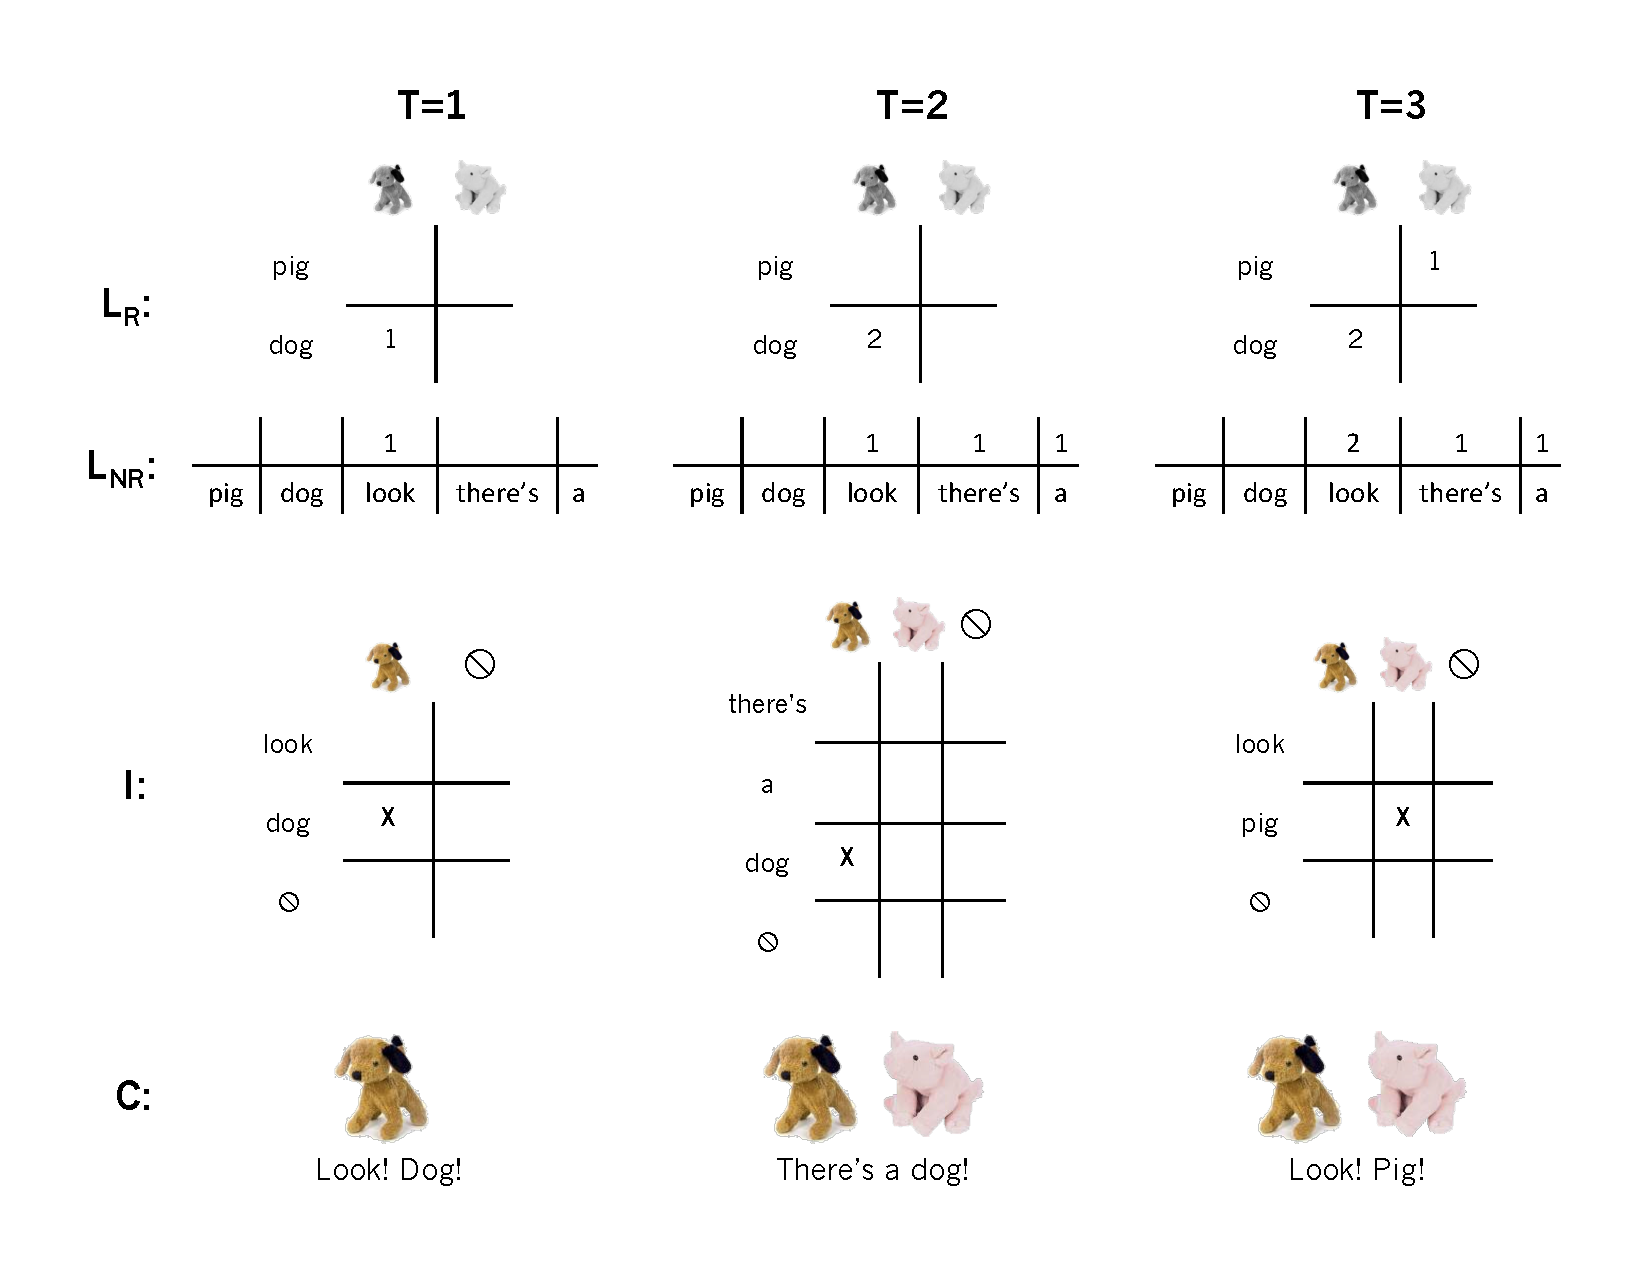
\includegraphics[width=6.25in]{figures/inference_diagram.pdf}
\caption{\label{fig:inference_diagram} A schematic of the model's evolving internal states when applied to a simple corpus with three contexts (marked $T=1,2,3$). States are shown for the particle filter inference algorithm with a single particle. Show at the top are the referential and non-referential lexicons (for simplicity, only the words ``pig'' and ``dog'' are shown in the referential lexicon). In the middle, the model's guesses about the referential correspondence between words and objects are shown for each situation.}
\end{center}
\end{figure}



\subsection{Batch learning}

In the full generative model the contexts are exchangeable: the order of contexts doesn't impact the overall probability. This means that we could always pretend a particular context was the last one. This idea gives rise to the \emph{Gibbs sampling} strategy: rather than building a sample incrementally as above, start with any assignment of $\vec{I}$ and $\vec{r}$ and then update by selecting a context, pretending it is the last, removing its counts and then re-sampling using the update described above. Sweeping through contexts updating in this way yields a Markov chain Monte Carlo sampling algorithm---independent of were we start the context variables, they will converge to a sample from the correct posterior.

\nnote{if we want to make the point that batch and incremental aren't so different, we should point out that the key property that let us derive both is that contexts (i.e. I and r) are independent given lexica, L. the conjugacy business just gives us a clean closed form for the, evolving, posterior on L. where should this discussion go?}


% for simplicity, we assume that there is a uniform prior over possible intentions (though we return to this issue in the Discussion). 
%
%Here is where our current model diverges from that of \citeA{frank2009}. In that work, we integrated across referential intentions and focused primarily on inferring the meanings of words in the absence of further interpretive information. In contrast, in the current model we focus on the process of incremental interpretation, and treat the lexicon as a byproduct of the process of interpretation. Accordingly, we integrate over all possible lexicons:
%
%\begin{equation}
%P( I| W, O) \propto \int_L{P(W | I, L) P(I | O) P(I)  P(L) }
%\end{equation}
%
%Similarly to the previous work, we define the lexicon $L$ as consisting of two separate parts. The referential lexicon $L_R$ is a set of integrated Dirichlet-Multinomial distributions, one for each object in the world. This distribution represents the posterior probability of a particular word, relative to that object. The non-referential lexicon $L_{NR}$ is an independent Dirichlet-Multinomial distribution that captures the use of other words that do not refer in the current context.
%
%\begin{equation}
%P(L) = \prod_{o \in W}{P(L_{R_o})} + P(L_{NR}).
%\end{equation}

 

% \begin{equation}
% P(W | I, L) = \gamma  
% \end{equation}

% intention, referential slot, and word vector
% for the referential word 

%$p(\vect{w} | I, R, L_R, L_{NR}) = p(w|O_i) * prod_{s \in S - S_r} {P(W_s | L_{NR})}$

%\subsection{Learning at the process level}
%
%
%\subsubsection{Batch inference using a gibbs sampler}
%
%\begin{equation}
%P_t(L|W_{1...t}, O_{1...t}) \propto P_{t-1}(L | ...) P(W_t, I_t, R_t | L)
%\end{equation}
%
%% prob of a particular sample under Dir-M is the same thing as the conjugate 
%% so you just get the conjugate update for each of the assignments 
%
%\subsubsection{Incremental inference using a particle filter}
%
%\begin{equation}
%P_t(L|W_{1...t}, O_{1...t}) \propto P_{t-1}(L | ...) P(I_t | W_t, O_t)
%\end{equation}

\section{Simulations}


\subsection{Corpus simulations}

We provide proof of concept that.
We make use of the Rollins Corpus from CHILDES \cite{macwhinney2000}, 

\subsection{Cross-situational word learning with adults}

\begin{figure}[h!]
\centering
% \begin{subfigure}{.5\textwidth}
%   \centering
  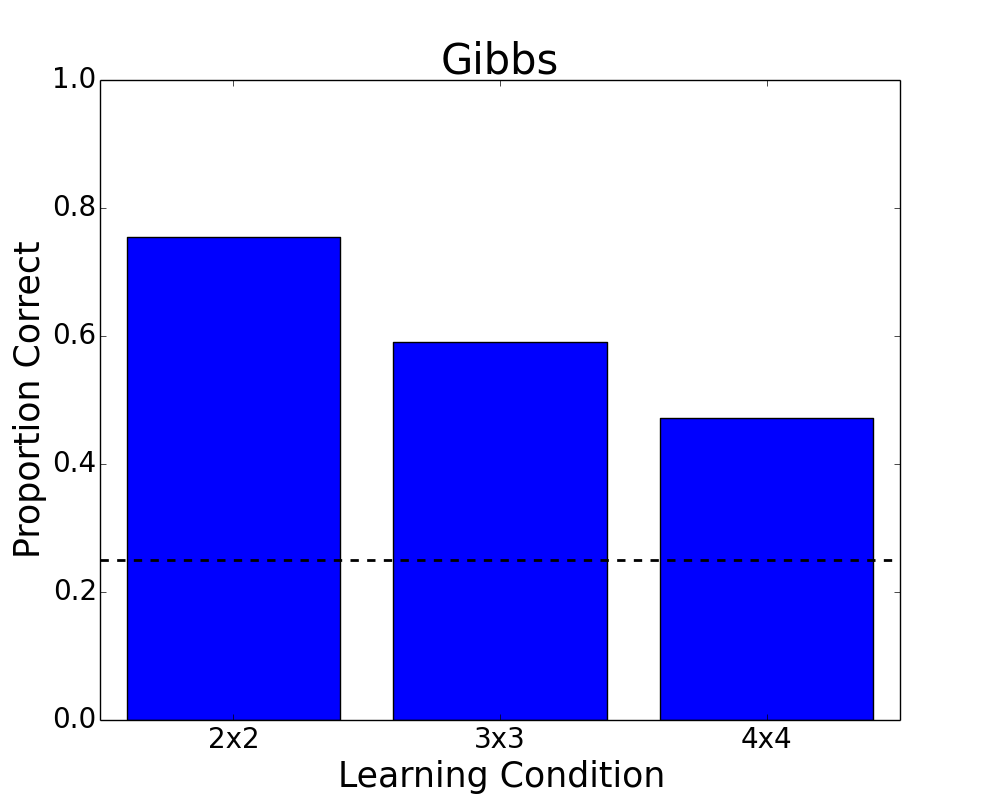
\includegraphics[width=3in]{figures/Gibbs.png}
% \end{subfigure}%
% \begin{subfigure}{.5\textwidth}
%   \centering
  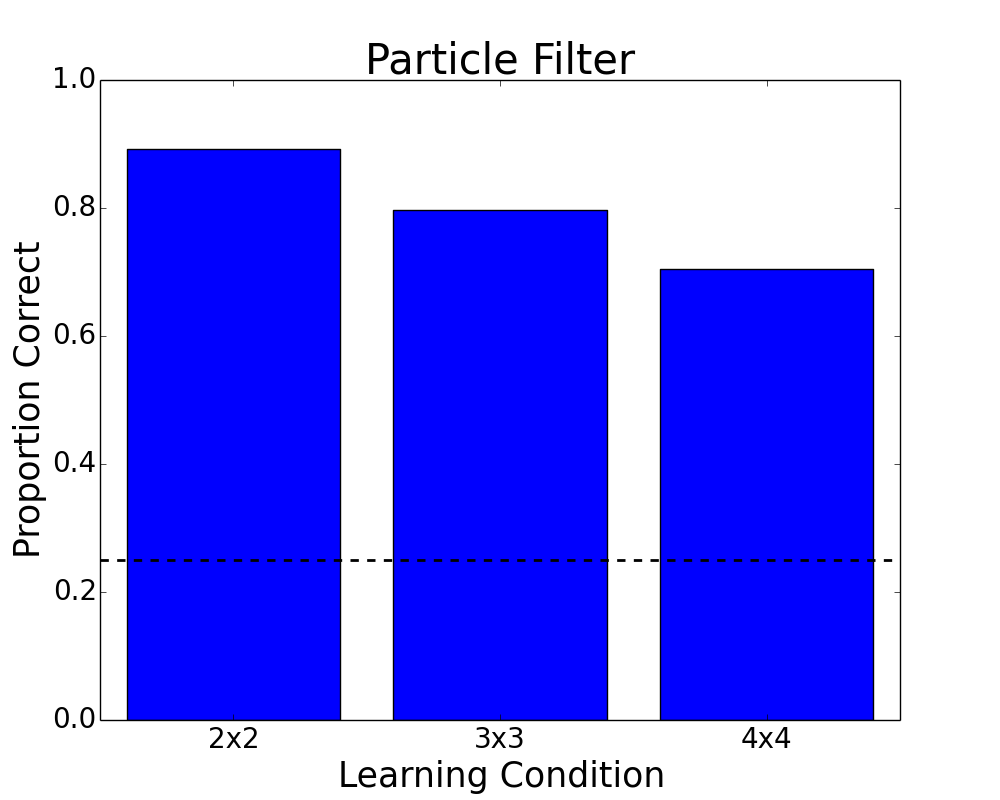
\includegraphics[width=3in]{figures/ParticleFilter.png}
% \end{subfigure}
\caption{Model predictions for the Yu and Smith (2007) stimuli. Proportion correct in a four alternative forced choice task is plotted as a function of the referential ambiguity condition. Performance is plotted for the Gibbs sampler (left) and incremental particle filter (right). For both inference algorithms, the model performs above chance on all conditions, and displays a graded decline in performance as the number of referential alternatives increases.}
\label{fig:yu2007sim}
\end{figure}

A key test of the model is its ability to learn word-object mappings across many individually ambiguous contexts. To evaluate the model's performance, we tested the model in a design identical to \citeA{yu2007b}. We presented the model with 18 novel words across many trials that were individually referentially ambiguous. A trial consisted of  {\it n} words presented with {\it n}  objects. As in \citeA{yu2007b}, we tested three values for  {\it n}: 2, 3, 4. For example, in an {\it n} = 2 condition, the model was presented with two words and two possible referents. Across conditions, the number of co-occurences of each word-object pairing was held constant. We evaluated the posterior lexicon using a Luce choice rule \cite{luce1959} for each word with four referential alternatives (one correct and three foils). 

Our model was able to successfully recover the correct mappings for most words. Because the lexicon is a continuous representation unlike the original model \cite{frank2009}, the model produced a graded pattern in performance in the test trials. As in the behavioral data \cite{yu2007b}, accuracy declined as the number of referential alternatives in the training trials increased: the model was most accurate in the {\it n} = 2 condition, and least accurate in the  {\it n}  = 4 condition (Fig.~\ref{fig:yu2007sim}). The particle filter inference algorithm performed overall better than the Gibbs sampler. 



\subsection{Experiments with children}

\subsubsection{Disambiguation}
Disambiguation is the behavioral bias for children to map novel words on  In the classic demonstrations of this phenomenon, children are presented with two objects, one familiar and one novel, and asked to This phenomenona is a particular

To simulate this result, we asked our model to determine the meaning of a 

\subsubsection{Dewar \& Xu (2007)}



\section{Discussion}



\subsection{Open questions for the cross-situational, social viewpoint}

\subsubsection{Synergies with other problems}

\subsubsection{Extensions to other parts of the vocabulary}

\subsubsection{Representations supporting cross-situational word learning}

\cite{yurovskyunderreview}

\subsection{Conclusions}

\newpage

\bibliographystyle{apacite}
\bibliography{dmww}

\end{document}

